\chapter{Военные корабли и их операторы}
\label{ch:ships-chapter}

Глава посвящена отечественным и зарубежным кораблям. Они могут иметь как военное, так и гражданское назначение. Гражданские суда используются в грузоперевозках, рыболовстве, туризме, разведке полезных ископаемых, спасательных работах, а также в спортивных, культурных и других целях. Для хранения информации о судах и других объектах ведутся базы знаний. Одной из таких баз знаний являются Викиданные. В этой главе изучены хранимык в Викиданных объекты кораблей и проведена оценке качества и полноты их описания.


\begin{marginfigure}[0.0cm]
  {
    \setlength{\fboxsep}{0pt}%
    \setlength{\fboxrule}{1pt}%
    \fcolorbox{gray}{gray}{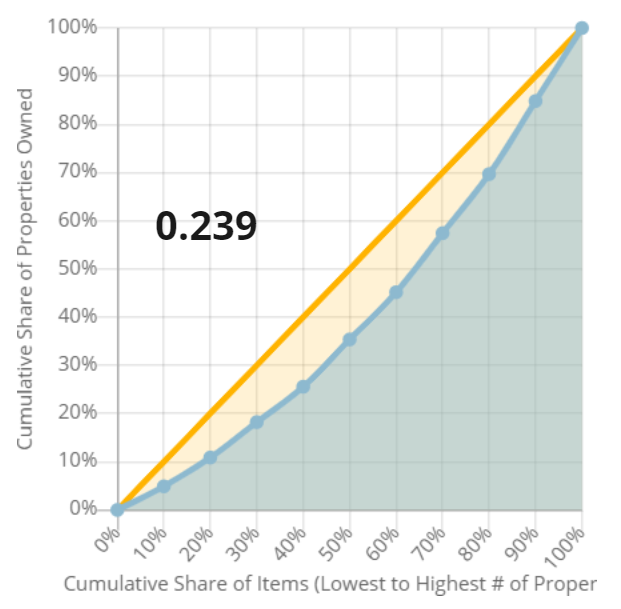
\includegraphics{chapter/ship/Russian_ships_topic_imbalance.png}}
  }
  \caption[График равномерности заполнения свойств объектов Викиданных.]{График равномерности заполнения по числу свойств объекта Викиданных \href{https://www.wikidata.org/wiki/Q11446}{корабль (Q11446)}, коэффициент Джини равен 0.239. Данные получены с помощью сервиса ProWD.id, 2020 год. График и коэффициент Джини показывают низкую равномерность заполнения свойств.}%
  \label{fig:prowd_ships-unbalanced}%
\end{marginfigure}


\section{Список кораблей}

\marginnote{
\href{https://www.wikidata.org/wiki/Q11446}{Корабль (Q11446)} -- это крупное морское судно.

Исследуемые свойства:
\begin{itemize}
  \item\href{https://www.wikidata.org/wiki/Property:P31}{Экземпляр (P31)}.
  \item\href{https://www.wikidata.org/wiki/Property:P137}{Оператор (P137)}.
  \item\href{https://www.wikidata.org/wiki/Property:P17}{Государство (P17)}.
  \item\href{https://www.wikidata.org/wiki/Property:P607}{Конфликт (P607)}
\end{itemize}
}

Построим список всех кораблей (см. листинг \ref{lst:ships_ru}).

\begin{lstlisting}[ language=SPARQL, caption={{\href{https://w.wiki/vjB}{Список кораблей}}\protect\footnotemark}, label=lst:ships_ru, ]
# List of ships
SELECT ?ship ?shipLabel
WHERE
{
  ?ship wdt:P31 wd:Q11446. # instance of ship
  SERVICE wikibase:label { bd:serviceParam wikibase:language "ru, en" }
}
\end{lstlisting}
\footnotetext{Найдено \num{19820} кораблей в 2017, \num{50681} в 2020, \numP{71203} в 2021. Ссылка на SPARQL-запрос: \href{https://w.wiki/vjB}{https://w.wiki/vjB}}

По данным ProWD больше всего свойств (34) имеет \href{https://www.wikidata.org/wiki/Q281147}{ледокол Красин (Q281147)}, а меньше всего свойству у корабля \href{https://www.wikidata.org/wiki/Q99198666}{Ливень (Q99198666)} (4 свойства) и корабля \href{https://www.wikidata.org/wiki/Q28155282}{Dispatch (Q28155282)} \cite{ProWD_ru_ships}.

Составим список кораблей, операторы которых находятся или находились в России, СССР или Российской империи (см. листинг \ref{lst:ships_with_ru_op}).

\begin{lstlisting}[ language=SPARQL, caption={\href{https://w.wiki/vjM}{Cписок кораблей, операторы которых находятся или находились в России, СССР или Российской Империи}}, label=lst:ships_with_ru_op ]
# List of ship from Russia, Soviet Union and Russian Empire
SELECT ?ship ?shipLabel
WHERE
{
  ?ship wdt:P31 wd:Q11446. # instance of ship
        wdt:P137/wdt:P17 ?country; 
    
  VALUES ?country {wd:Q34266 # Russian EMpire
                   wd:Q15180 # Soviet Union
                   wd:Q159}  # Russia
  SERVICE wikibase:label { bd:serviceParam wikibase:language "ru, en" }
}
\end{lstlisting}
\footnotetext{Найдено 579 кораблей в 2020 году, 578 кораблей в 2021 году. Ссылка на SPARQL-запрос: \href{https://w.wiki/vjM}{https://w.wiki/vjM}}


\section{Полнота Викиданных}

\label{question:ship_1}
\marginnote{Найти <<корабль Гиннесса>>. На выбор: самый большой, самый длинный, самый вместительный и т. д. Ответ можно найти на странице~\pageref{answer:ship_1}.}

Поиск точного количества кораблей в мире — трудная задача. Ведь данные о некоторых из них являются совершенно секретными, какие-то же — это частные судна и информации о них тоже нет. Предположим, что общее число кораблей примерно равно \num{1600000}, как указано в базе данных судов \cite{FleetMon}. На 2021 год было найдено только \num{71206} записей, что составило только 4,3\% от общего числа кораблей.


Что касается российских кораблей, в состов российский военных и гражданских флотов входит \num{17657} кораблей \cite{RussianShips}. В это же время скрипт в листинге \ref{lst:ships_with_ru_op} показывает лишь 578 кораблей, что составляет 3.23\% от общего числа российских кораблей. 

В обоих случаях разница между фактическим количеством кораблей и результатом запросов огромная, что говорит о неполноте Викиданных.


\label{question:ship_2}
\marginnote{На рисунке \ref{fig:grem_question} представлен самый известный советский \ruwiki{vgD}{эскадренный миноносец} \ruwiki{vgC}{проекта 7}, удостоенный звания <<гвардейский>>, назовите его.  Ответ можно найти на странице~\pageref{answer:ship_2}.}

\begin{marginfigure}[0.0cm]
  {
    \setlength{\fboxsep}{0pt}%
    \setlength{\fboxrule}{1pt}%
    \fcolorbox{gray}{gray}{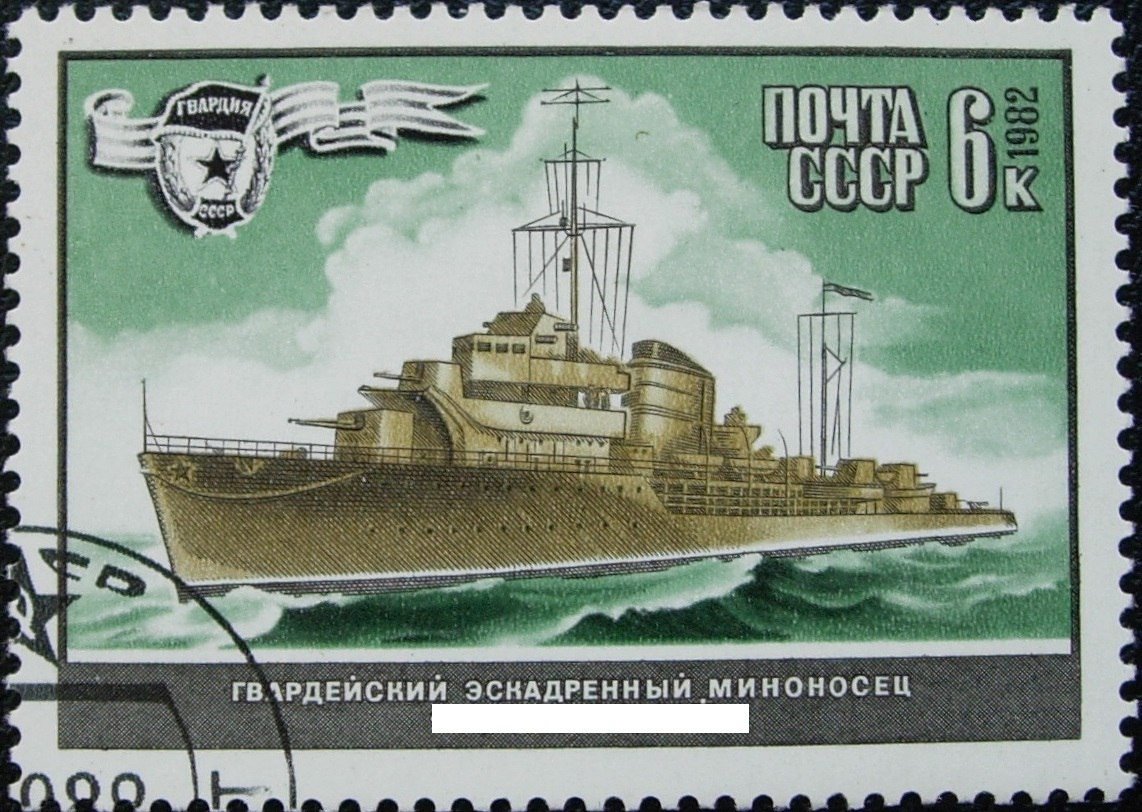
\includegraphics{chapter/ship/Secret_Grem_ship.jpg}}
  }
  \caption[Известный советский миноносец.]{Почтовая марка, на которой изображен известный советский \ruwiki{vgD}{эскадренный миноносец} \ruwiki{vgC}{проекта 7}.}%
  \label{fig:grem_question}%
\end{marginfigure}

\section{Полнота свойств объектов военных кораблей}

Составим список кораблей, участвовавших в каких-либо конфликтах (см. листинг \ref{lst:ships_in_conflict_ru}).

\begin{lstlisting}[ language=SPARQL, caption={{\href{https://w.wiki/vjN}{Список кораблей, участвовавших в каких-либо конфликтах}}\protect\footnotemark}, label=lst:ships_in_conflict_ru, ]
# List of ships with countries and war conflicts
SELECT ?ship ?shipLabel ?countryLabel ?conflict ?conflictLabel
WHERE
{
  ?ship wdt:P31 wd:Q11446;        # instance of ship
        wdt:P137/wdt:P17 ?country;# belongs to country
        wdt:P607 ?conflict.       # engaged in some conflict
  SERVICE wikibase:label { bd:serviceParam wikibase:language "ru, en" }
}
\end{lstlisting}
\footnotetext{Найдено \num{3586} кораблей в 2020 году, \num{3567} в 2021 году. Ссылка на SPARQL-запрос: \href{https://w.wiki/vjN}{https://w.wiki/vjN}}

У военных кораблей, участвовавших в конфликтах, указывается свойство \href{https://www.wikidata.org/wiki/Property:P607}{conflict (P607)} (война/сражение). В то же время военные конфликты и военные операции, которые являются частью войн, являются разными понятиями. Объекты кораблей можно условно по делить на два типа:

\begin{enumerate}
  \item Объекты, у которых военные операции объединены с военными конфликтами. Например, у \href{https://www.wikidata.org/wiki/Q4148613}{эсминца Гремящий} 10 войн/сражений, см. листинг \ref{lst:grem_wars}. Такое большое число связано с тем, что корабль принял участие во многих \href{https://ru.wikipedia.org/wiki/Арктические_конвои}{арктических конвоях}, которые являются военными операциями.
  \item Объекты, у которых военные операции отделены от военных конфликтов. Например, у британского крейсера \href{https://ru.wikipedia.org/wiki/HMS_Trinidad_(1940)}{HMS Trinidad} участие в военной кампании и арктическом конвое указаны как часть Второй мировой войны с помощью квалификатора \href{https://www.wikidata.org/wiki/Property:P1012}{including (P1012)}. Таким образом, в Викиданных у этого крейсера указана одна война/сражение.
\end{enumerate}


\label{question:ship_3}
\marginnote{Вывести фотографии тех кораблей, про которые снимали кино. Если таких не найдётся, тогда те корабли, о которых писали в книгах. Ответ можно найти на странице~\pageref{answer:ship_3}}


\begin{lstlisting}[ language=SPARQL, caption={{\href{https://w.wiki/vjP}{Военные конфликты, в которых участвовал \href{https://www.wikidata.org/wiki/Q4148613}{эсминец Гремящий}}}\protect\footnotemark}, label=lst:grem_wars, ]
SELECT ?conflict ?conflictLabel
WHERE
{
  ?ship wdt:P31 wd:Q11446;
        wdt:P607 ?conflict.
    
  FILTER (?ship IN (wd:Q4148613))
              
  SERVICE wikibase:label { bd:serviceParam wikibase:language "ru, en" }
}
\end{lstlisting}
\footnotetext{Найдено \num{10} конфликтов, 2021 год. Ссылка на SPARQL-запрос: \href{https://w.wiki/vjP}{https://w.wiki/vjP}}

Для первого типа объектов в скриптах с поиском у кораблей свойства \href{https://www.wikidata.org/wiki/Property:P607}{conflict (P607)} будет отображаться больше войн/сражений, чем при втором. Но в этом случае операция \href{https://ru.wikipedia.org/wiki/Одесская_оборона_(1941)}{Одесская оборона} будет стоять наряду с \href{https://ru.wikipedia.org/wiki/Великая_Отечественная_война}{Великой Отечественной войной}, хотя она является частью этой войны. В такой ситуации выводимые данные будут не точными.

Составим список кораблей (на русском языке) России, СССР или Российской Империи, участвовавших в каких-либо конфликтах (см. листинг \ref{lst:ships_in_war_ru}).

\begin{lstlisting}[ language=SPARQL, caption={{\href{https://w.wiki/vjR}{Список кораблей России, СССР или Российской Империи, участвовавших в каких-либо конфликтах}}\protect\footnotemark}, label=lst:ships_in_war_ru, ]
#List of ship with countries and war conflicts
SELECT ?ship ?shipLabel ?countryLabel ?conflict ?conflictLabel
WHERE
{
  ?ship wdt:P31 wd:Q11446;        # instance of ship
        wdt:P137/wdt:P17 ?country;        # belongs to operator
        wdt:P607 ?conflict.       # engaged in some conflict
  
  VALUES ?country {wd:Q34266 # Russian EMpire
                   wd:Q15180 # Soviet Union
                  wd:Q159}  # Russia

  SERVICE wikibase:label { bd:serviceParam wikibase:language "ru, en" }
}
\end{lstlisting}
\footnotetext{Найдено \num{86} кораблей в 2020 году, \num{82} корабля в 2021 году. Ссылка на SPARQL-запрос: \href{https://w.wiki/vjR}{https://w.wiki/vjR}}

При анализе результатов работы скрипта в листинге \ref{lst:ships_in_war_ru} важно заметить, что попавшие в него корабли не обязательно связанны только с Россией, СССР или Российской империей. Например, корабль \href{https://www.wikidata.org/wiki/Q653477}{Kasato Maru (Q653477)} -- японский, однако, в списке его операторов указано несколько значений. Среди них есть \href{https://www.wikidata.org/wiki/Q3737187}{Добровольный флот (Q3737187)}, который также владел этим кораблем. Это значит, что один и тот же корабль в различные периоды времени может принадлежать разным операторам, переходить от владельца в владельцу.

  
\begin{figure*}[ht]
  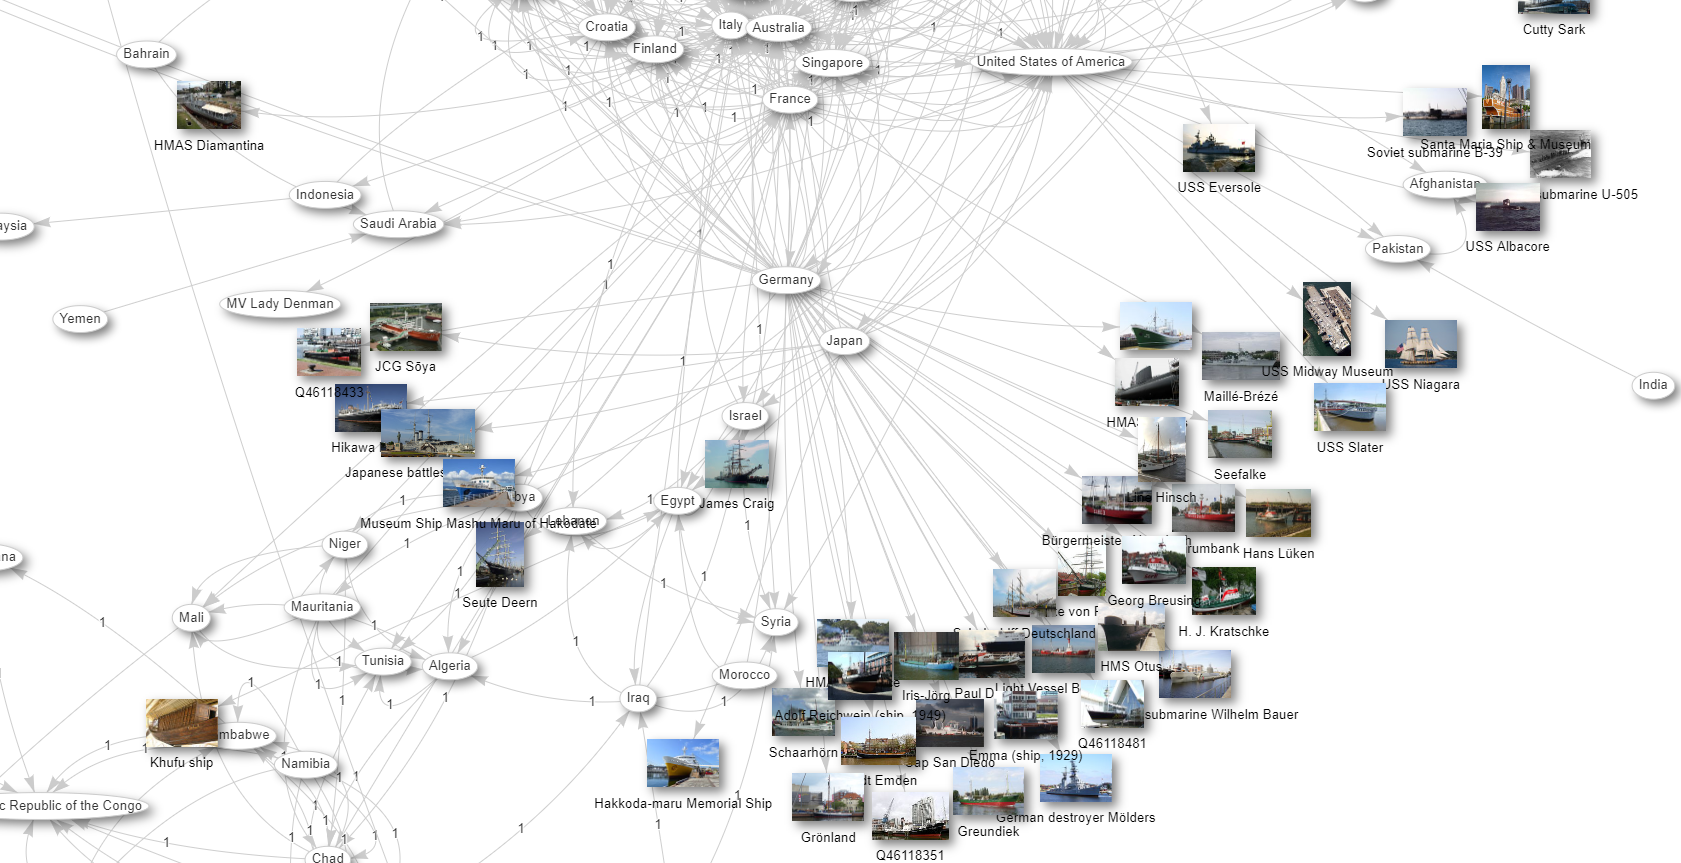
\includegraphics[width=0.9\linewidth]{chapter/ship/museum_graph.png}
  \caption[Граф стран и кораблей-музеев]{Фрагмент графа стран, кораблей-музеев и конфликтов, построенный по скрипту в листинге \ref{lst:museum_graph}.}%
  \label{fig:museum_graph}%
\end{figure*}
\section{Корабли-музеи в странах мира}

\href{https://www.wikidata.org/wiki/Q575727}{Корабль-музей (Q575727)} -- корабль, на котором размещена музейная экспозиция, посвященная истории корабля. Такие корабли используются в общеобразовательных и мемориальных целях. Участие корабля в \href{https://www.wikidata.org/wiki/Q180684}{военном конфликте (Q180684)} может послужить поводом для создания корабля-музея в память о прошедших событиях. 

Построим граф кораблей-музеев и стран, в которых эти корабли находятся. Вершинами графа являются \href{https://www.wikidata.org/wiki/Q6256}{страны (Q6256)} и \href{https://www.wikidata.org/wiki/Q575727}{корабли-музеи (Q575727)}. Ребро между кораблем и страной означает, что корабль находится в этой стране. А ребро между двумя странами означает, что между этими странами были конфликты, число которых равно весу ребра. Скрипт в листинге \ref{lst:museum_graph} строит граф по описанным выше правилам.

\begin{lstlisting}[ language=SPARQL, caption={{\href{https://w.wiki/vfj}{Граф кораблей-музеев и стран, в которых они находятся.}}\protect\footnotemark}, label=lst:museum_graph, ]
#defaultView:Graph    
SELECT ?vertex1 ?vertex1Label ?vertex2 ?vertex2Label ?edgeLabel ?image 
WHERE {
  {
    # Conflicts
    SELECT ?vertex1 ?vertex1Label ?vertex2 ?vertex2Label 
            (STR(COUNT(?conflict)) as ?edgeLabel) 
    WHERE
    {
      ?conflict wdt:P31 wd:Q180684 .
      ?conflict wdt:P710 ?vertex1, ?vertex2 .
      ?vertex1 wdt:P31 wd:Q6256 . 
      ?vertex2 wdt:P31 wd:Q6256

      FILTER (?vertex1 != ?vertex2 && STR(?vertex1) < STR(?vertex2))
    
      SERVICE wikibase:label { bd:serviceParam wikibase:language "en" }
    }
    GROUP BY ?vertex1 ?vertex1Label ?vertex2 ?vertex2Label
  }
  UNION
  {
    # Museum ships
SELECT DISTINCT ?vertex1 ?vertex1Label ?vertex2 ?vertex2Label ?image
    WHERE
    {
      ?vertex2 wdt:P31 wd:Q575727 .
      {?vertex2 wdt:P17 ?vertex1} UNION # located in country
      {?vertex2 wdt:P131/wdt:P17 ?vertex1}
        
      OPTIONAL { ?vertex2 wdt:P18 ?image}
        
      SERVICE wikibase:label { bd:serviceParam wikibase:language "en"}
    }
  }
}
\end{lstlisting}
\footnotetext{Найдено 117 вершин графа в 2021 году. Ссылка на SPARQL-запрос: \href{https://w.wiki/vfj}{https://w.wiki/vfj}.}

Из фрагмента графа на рисунке \ref{fig:museum_graph} видно, что корабли-музеи по большей части принадлежат Германии, США и Австралии. Такая <<корреляция>> вполне логична, так как данные страны имеют длительную историю, за которую они поучаствовали во многих военных конфликтах. Также эти страны имеют выход к морю, что исторически обуславливает наличие у них флота, в котором могут найтись корабли для создания музея.


\begin{figure*}[ht]
  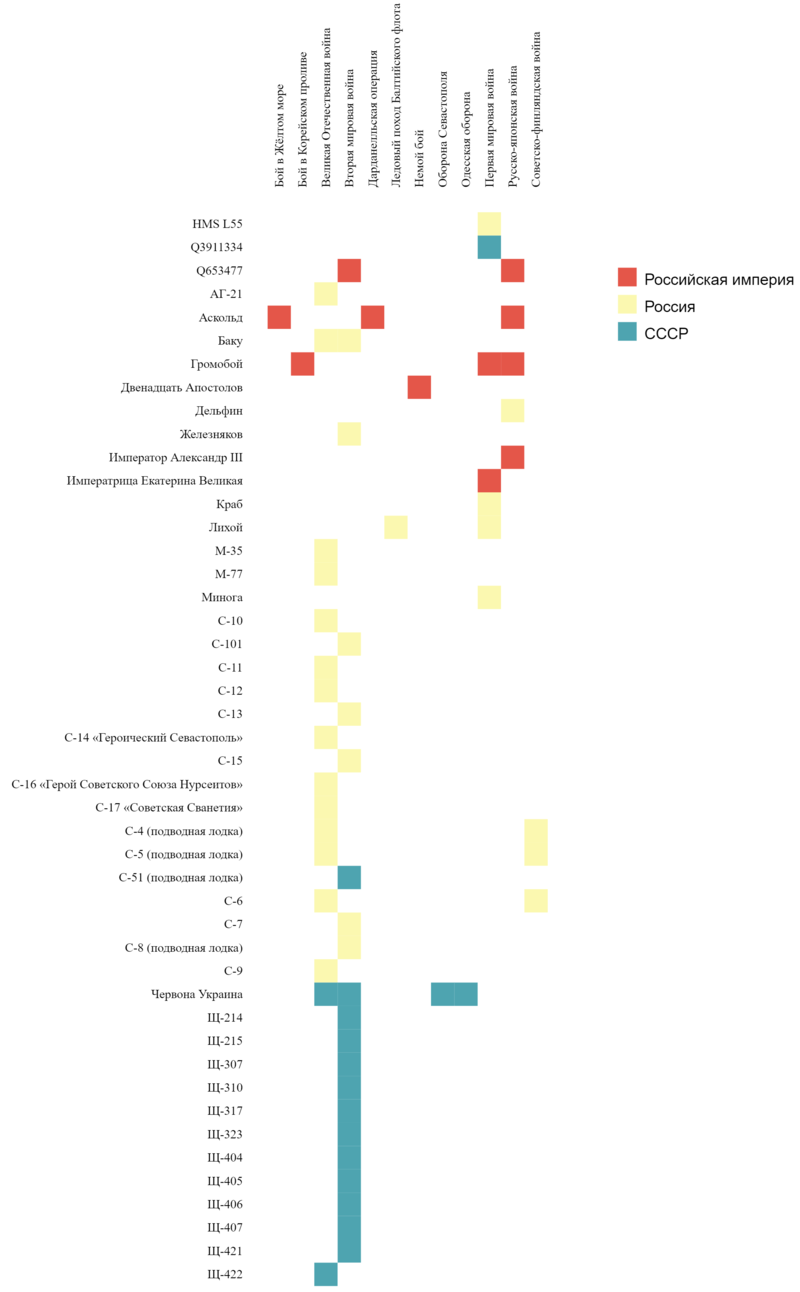
\includegraphics[width=0.95\linewidth]{chapter/ship/Ships_by_country_and_conflict_ru.png}
  \caption[Список кораблей и конфликтов, в которых они участвовали]{Фрагмент cписка кораблей, связанных с Россией и участвовавших в военных конфликтах, 2017 год. Из списка видно, что больше большая часть кораблей связаны с Россией и СССР, а также со Второй мировой или Великой Отечественной войнами.}%
  \label{fig:ships_by_country_and_conflict}%
\end{figure*}